\documentclass[12pt]{amsart}
\usepackage[letterpaper, portrait, left = 1in, right = 1in, top = 1.2in, bottom=1.5in]{geometry} 
%\usepackage{setspace} \doublespacing
%\usepackage[letterpaper, portrait, margin=1.3in]{geometry}
\usepackage[table,xcdraw]{xcolor}
\usepackage{amssymb}
\usepackage{amsfonts}
\usepackage{longtable}
\usepackage{amsmath,amsthm}
\usepackage{enumitem}
\usepackage[utf8]{inputenc}
\usepackage{mathtools}
\usepackage{graphicx}
\usepackage{parskip}
\usepackage{multicol}
\usepackage{listings}
\usepackage[skip=0.25pt]{caption}
\usepackage[mathscr]{euscript}
\usepackage{quiver}
\setlength{\parindent}{0pt}
\usepackage{thm-restate}
\definecolor{vividburgundy}{rgb}{0.62, 0.11, 0.21}
\usepackage[driverfallback=hypertex,pagebackref=false,colorlinks,citecolor=vividburgundy]{hyperref}
\usepackage[capitalize]{cleveref}
%\usepackage[cmintegrals,cmbraces]{newtxmath}
%\usepackage{ebgaramond-maths}

%\usepackage{fourier}
%----------FONT OPTIONS----------
% sans-serif
%\usepackage[sfdefault]{FiraSans}
 %\usepackage[sfdefault]{roboto}
% \usepackage[sfdefault]{noto-sans}
%\usepackage[default]{sourcesanspro}

% serif
%\usepackage{CormorantGaramond}

%\usepackage{charter}
\usepackage[T1]{fontenc}
\usepackage{cleveref}
\definecolor{dg}{RGB}{10, 100, 10}
\setlength{\parindent}{0in}
\renewcommand{\qed}{$\hfill\blacksquare$}
% \newtheoremstyle{style}{2pt}{1pt}{\normalfont}{}{\bfseries}{\\}{0cm}{}
% \theoremstyle{style}
\newtheorem{lemma}{Lemma}[section]
% \newtheorem{lemma}{Lemma}
\newtheorem{thm}[lemma]{Theorem}
\newtheorem{prop}[lemma]{Proposition}
\newtheorem{cor}[lemma]{Corollary}
\newtheorem{conj}[lemma]{Conjecture}
\newtheorem{cl}[lemma]{Claim}
\newtheorem{rmk}{Remark}
\newtheorem{defn}[lemma]{Definition}
\newtheorem{qs}{Question}
\newtheoremstyle{styleS}{}{}{\color{dg}}{}{\color{dg}\bfseries}{. }{0cm}{}
\theoremstyle{styleS}
\newtheorem*{sol}{Solution}
\newtheoremstyle{style1}{}{}{\normalfont}{}{\bfseries}{. }{0cm}{}
\theoremstyle{style1}
\newtheorem{prob}{Problem}[section]
\newtheorem*{prb}{Problem}
\newtheoremstyle{style2}{1pt}{4pt}{\normalfont}{}{\itshape}{. }{0cm}{}
\theoremstyle{style2}
\newtheorem{ex}[lemma]{Example}
\newtheorem*{pf}{Proof}

\newcommand{\norm}[2]{
\left\lVert #1 \right\rVert_{#2}
}
\usepackage{mathrsfs}
%\usepackage[table,xcdraw]{xcolor}
\usepackage{booktabs}
\usepackage{tikz}
\usetikzlibrary{matrix}
\renewcommand{\l}{\ell}


\newcommand{\fA}{{\mathfrak{A}}}   \newcommand{\fB}{{\mathfrak{B}}}
\newcommand{\fC}{{\mathfrak{C}}}   \newcommand{\fD}{{\mathfrak{D}}}
\newcommand{\fE}{{\mathfrak{E}}}   \newcommand{\fF}{{\mathfrak{F}}}
\newcommand{\fG}{{\mathfrak{G}}}   \newcommand{\fH}{{\mathfrak{H}}}
\newcommand{\fI}{{\mathfrak{I}}}   \newcommand{\fJ}{{\mathfrak{J}}}
\newcommand{\fK}{{\mathfrak{K}}}   \newcommand{\fL}{{\mathfrak{L}}}
\newcommand{\fM}{{\mathfrak{M}}}   \newcommand{\fN}{{\mathfrak{N}}}
\newcommand{\fO}{{\mathfrak{O}}}   \newcommand{\fP}{{\mathfrak{P}}}
\newcommand{\fQ}{{\mathfrak{Q}}}   \newcommand{\fR}{{\mathfrak{R}}}
\newcommand{\fS}{{\mathfrak{S}}}   \newcommand{\fT}{{\mathfrak{T}}}
\newcommand{\fU}{{\mathfrak{U}}}   \newcommand{\fV}{{\mathfrak{V}}}
\newcommand{\fW}{{\mathfrak{W}}}   \newcommand{\fX}{{\mathfrak{X}}}
\newcommand{\fY}{{\mathfrak{Y}}}   \newcommand{\fZ}{{\mathfrak{Z}}}

\newcommand{\cA}{{\mathcal{A}}}   \newcommand{\cB}{{\mathcal{B}}}
\newcommand{\cC}{{\mathcal{C}}}   \newcommand{\cD}{{\mathcal{D}}}
\newcommand{\cE}{{\mathcal{E}}}   \newcommand{\cF}{{\mathcal{F}}}
\newcommand{\cG}{{\mathcal{G}}}   \newcommand{\cH}{{\mathcal{H}}}
\newcommand{\cI}{{\mathcal{I}}}   \newcommand{\cJ}{{\mathcal{J}}}
\newcommand{\cK}{{\mathcal{K}}}   \newcommand{\cL}{{\mathcal{L}}}
\newcommand{\cM}{{\mathcal{M}}}   \newcommand{\cN}{{\mathcal{N}}}
\newcommand{\cO}{{\mathcal{O}}}   \newcommand{\cP}{{\mathcal{P}}}
\newcommand{\cQ}{{\mathcal{Q}}}   \newcommand{\cR}{{\mathcal{R}}}
\newcommand{\cS}{{\mathcal{S}}}   \newcommand{\cT}{{\mathcal{T}}}
\newcommand{\cU}{{\mathcal{U}}}   \newcommand{\cV}{{\mathcal{V}}}
\newcommand{\cW}{{\mathcal{W}}}   \newcommand{\cX}{{\mathcal{X}}}
\newcommand{\cY}{{\mathcal{Y}}}   \newcommand{\cZ}{{\mathcal{Z}}}

\newcommand{\sA}{{\mathscr{A}}}   \newcommand{\sB}{{\mathscr{B}}}
\newcommand{\sC}{{\mathscr{C}}}   \newcommand{\sD}{{\mathscr{D}}}
\newcommand{\sE}{{\mathscr{E}}}   \newcommand{\sF}{{\mathscr{F}}}
\newcommand{\sG}{{\mathscr{G}}}   \newcommand{\sH}{{\mathscr{H}}}
\newcommand{\sI}{{\mathscr{I}}}   \newcommand{\sJ}{{\mathscr{J}}}
\newcommand{\sK}{{\mathscr{K}}}   \newcommand{\sL}{{\mathscr{L}}}
\newcommand{\sM}{{\mathscr{M}}}   \newcommand{\sN}{{\mathscr{N}}}
\newcommand{\sO}{{\mathscr{O}}}   \newcommand{\sP}{{\mathscr{P}}}
\newcommand{\sQ}{{\mathscr{Q}}}   \newcommand{\sR}{{\mathscr{R}}}
\newcommand{\sS}{{\mathscr{S}}}   \newcommand{\sT}{{\mathscr{T}}}
\newcommand{\sU}{{\mathscr{U}}}   \newcommand{\sV}{{\mathscr{V}}}
\newcommand{\sW}{{\mathscr{W}}}   \newcommand{\sX}{{\mathscr{X}}}
\newcommand{\sY}{{\mathscr{Y}}}   \newcommand{\sZ}{{\mathscr{Z}}}

\newcommand{\ta}{{\tilde{a}}}   \newcommand{\tb}{{\tilde{b}}}
\newcommand{\tc}{{\tilde{c}}}   \newcommand{\td}{{\tilde{d}}}
\newcommand{\te}{{\tilde{e}}}   \newcommand{\tf}{{\tilde{f}}}
\newcommand{\tg}{{\tilde{g}}}   
\newcommand{\ti}{{\tilde{i}}}   \newcommand{\tj}{{\tilde{j}}}
\newcommand{\tk}{{\tilde{k}}}   \newcommand{\tl}{{\tilde{l}}}
\newcommand{\tm}{{\tilde{m}}}   \newcommand{\tn}{{\tilde{n}}}
		         	\newcommand{\tp}{{\tilde{p}}}
\newcommand{\tq}{{\tilde{q}}}   \newcommand{\tr}{{\tilde{r}}}
\newcommand{\ts}{{\tilde{s}}}   
\newcommand{\tu}{{\tilde{u}}}   \newcommand{\tv}{{\tilde{v}}}
\newcommand{\tw}{{\tilde{w}}}   \newcommand{\tx}{{\tilde{x}}}
\newcommand{\ty}{{\tilde{y}}}   \newcommand{\tz}{{\tilde{z}}}

\newcommand{\red}{{\color{red}red}}
\newcommand{\blue}{{\color{blue}blue}}

\newcommand{\into}{\hookrightarrow}
\newcommand{\onto}{\twoheadrightarrow}
\newcommand\N{\ensuremath{\mathbb{N}}}

%\newcommand\L{\ensuremath{\mathbb{L}}}
\newcommand{\bP}{\mathbb{P}}
\newcommand\M{\ensuremath{\mathbb{M}}}
\newcommand\R{\ensuremath{\mathbb{R}}}
\newcommand\Z{\ensuremath{\mathbb{Z}}}
\renewcommand\O{\ensuremath{\emptyset}}
\newcommand\Q{\ensuremath{\mathbb{Q}}}
\newcommand\C{\ensuremath{\mathbb{C}}}
\newcommand{\K}{\ensuremath{\mathbb{K}}}
\newcommand\F{\ensuremath{\mathbb{F}}}
\newcommand{\aff}{\ensuremath{\mathbb{A}}}
\newcommand{\proj}{\ensuremath{\mathbb{P}}}
\newcommand{\dd}{\mathrm{d}}
\newcommand{\m}{\ensuremath{\mathfrak{m}}}
\newcommand{\p}{\ensuremath{\mathfrak{p}}}
\newcommand{\n}{\ensuremath{\mathfrak{n}}}
\renewcommand{\phi}{\varphi}
\renewcommand{\qedsymbol}{\ensuremath{\blacksquare}}
%\newcommand{\st}{\;|\;}
\newcommand{\st}{%
  \nonscript\;
  \ifnum\currentgrouptype=16
    \;\middle|\;
  \else
    \;|\;
  \fi
  \nonscript\;}
\newcommand{\ltr}{\par \noindent \framebox[1\width]{ $\implies$ } \hspace{.2cm}}
\newcommand{\rtl}{\par \noindent \framebox[1\width]{ $\impliedby$ } \hspace{.2cm} }
\newcommand{\abs}[1]{\left| #1 \right|}
\newcommand{\inner}[2]{\left\langle #1, #2 \right\rangle}
\newcommand{\E}[1]{\mathbb E\left[ #1 \right]}
\newcommand{\e}[1]{\exp\left( #1 \right)}
\renewcommand{\P}[1]{\mathbb P\left[ #1 \right]}
\newcommand{\Var}[1]{\text{Var}\left[ #1 \right]}
\newcommand*\circled[1]{\tikz[baseline=(char.base)]{
            \node[shape=circle,draw,inner sep=2pt] (char) {#1};}}
\newcommand{\ds}{\displaystyle}

\DeclareMathOperator{\sym}{Sym}
\DeclareMathOperator{\mds}{MDS}
\DeclareMathOperator{\Tor}{Tor}
\DeclareMathOperator{\Ext}{Ext}
\DeclareMathOperator{\adj}{adj}
\DeclareMathOperator{\Tr}{Tr}
\DeclareMathOperator{\GL}{GL}
%\DeclareMathOperator{\Tr}{Tr}
\DeclareMathOperator{\orbit}{Or}
\DeclareMathOperator{\stab}{Stab}
\DeclareMathOperator{\fix}{Fix}
\DeclareMathOperator{\re}{Re}
\DeclareMathOperator{\im}{Im}
\DeclareMathOperator{\ord}{Ord}
\DeclareMathOperator{\mspec}{mSpec}
\DeclareMathOperator{\spec}{Spec}
\DeclareMathOperator{\frob}{Frob}
\DeclareMathOperator{\id}{Id}
\DeclareMathOperator{\colim}{colim}
\DeclareMathOperator{\loc}{loc}
\DeclareMathOperator{\res}{Res}
\DeclareMathOperator{\rad}{rad}
\DeclareMathOperator{\Res}{Res}
\DeclareMathOperator{\diam}{diam}
\DeclareMathOperator{\arcsec}{arcsec}
\DeclareMathOperator{\arccot}{arccot}
\DeclareMathOperator{\len}{len}
\DeclareMathOperator{\area}{area}
\DeclareMathOperator{\vol}{vol}
\DeclareMathOperator{\ev}{ev}
\DeclareMathOperator{\sgn}{sgn}
\DeclareMathOperator{\supp}{supp}
\DeclareMathOperator{\diff}{d}
\DeclareMathOperator{\Dom}{Dom}
\DeclareMathOperator{\rk}{rank}
\renewcommand{\d}{\diff}
\let\oldend\endlinechar
\renewcommand{\endlinechar}{\oldend}
\newcommand{\open}{\underset{\text{open}}{\subset}}
\newcommand{\divides}{\mathbin{|}}
\newcommand{\set}[1]{\ensuremath{\left\{#1\right\}}}
\newcommand{\sett}{\coloneqq}
\newcommand*\isomap{%
  \xrightarrow{\raisebox{-0.9ex}[0ex][0ex]{$\sim$}}%
}
\renewcommand{\epsilon}{\varepsilon}
\newcommand{\fa}{~\forall~}
%\usepackage[nobottomtitles*]{titlesec}
\usepackage{titletoc}
%\titleformat{\section}[runin]
%{\normalfont\Large\bfseries}
%{}{0pt}{}%
%[\ifthenelse{\equal{\thesection}{0}}{\\\vspace*{0pt}}{\space\thesection}]
\newcommand{\sint}{\sin\theta}
\newcommand{\cost}{\cos\theta}
\newcommand{\tant}{\tan\theta}
\newcommand{\lb}{\left[}
\newcommand{\rb}{\right]}
\newcommand{\lp}{\left(}
\newcommand{\rp}{\right)}
\newcommand{\br}[1]{\lb#1\rb}
\newcommand{\pa}[1]{\lp#1\rp}
\usepackage{pdfpages}
\usepackage{fancyhdr}
	\pagestyle{fancyplain}
	\fancyhf{}
	\fancyhead[C]{\thepage}

\usepackage{wrapfig}
\usepackage{multicol}
\usepackage[breakable]{tcolorbox}
%\fontfamily{qcr}\selectfont 
%\usepackage[backend=bibtex]{biblatex}
\usepackage[
backend=biber,
style=alphabetic,%firstinits,
citestyle=ieee-alphabetic,
%natbib=true,
%uniquelist=false,
maxnames=10,
sorting=ynt
]{biblatex}
%\addbibresource{writeup/article/refs.bib}
%\title{\vspace{-1cm}}
\title{\textbf{CONVEX AND CONIC OPTIMIZATION}\\ Homework $4$}
\usepackage{quiver}
\usepackage[nobottomtitles*]{titlesec}
\usepackage{titletoc}
\titleformat{\section}[runin]
  {\normalfont\Large\bfseries}
  {}{0pt}{}%
  [\ifthenelse{\equal{\thesection}{0}}{\\\vspace*{0pt}}{\space\thesection}]
\author{{\Large NILAVA METYA} \\ 
\href{mailto:nilava.metya@rutgers.edu}{nilava.metya@rutgers.edu}\\
\href{mailto:nm8188@princeton.edu}{nm8188@princeton.edu}}
\date{April $4$, $2024$}
\newcommand{\pb}{\section{Problem}~\par}
\newcommand{\soln}{\subsection*{Solution}}
\newcommand{\conv}{\text{conv}}
\newcommand{\epi}{\text{epi}}
\usepackage{pdfpages}
\usepackage{fancyhdr}
	\pagestyle{fancyplain}
	\fancyhf{}
	\fancyhead[R]{\thepage}
\setlength{\columnsep}{1.2cm}
\newcommand{\fa}{~\forall}
\begin{document}

\maketitle

\pb
The nuclear norm of a matrix $A\in\R^{m\times n}$ is defined by $$\norm A\ast \sett \sum_{i=1}^{\min\set{m,n}}\sigma_{i}(A).$$
\begin{enumerate}[leftmargin=*]
\item Show that the dual norm of the spectral norm is the nuclear norm.
\item Show that the problem of minimizing the nuclear norm of a matrix subject to arbitrary affine constraints can be cast as a semidefinite program.
\end{enumerate}

\soln

\begin{enumerate}[leftmargin=*]
\item Let $\norm{\cdot}{}$ denote the spectral norm here, and let the nuclear norm be $\norm{\cdot}{*}$. By definition, $\ds\norm{A}{*} = \max_{\substack{\norm{C}{}\le 1 \\ C\in \R^{m\times n}}} \Tr(C^{\top}A)$. For each matrix $X\in\R^{m\times n}$, denote it's singular values by $\sigma_{1}(X) \ge \sigma_{2}(X)\ge \cdots \ge \sigma_{\min\set{m,n}}(X)$ in non-increasing order. 

\textbf{Lower bound on nuclear norm:} Let $A = U\Sigma V^{\top}$ be the SVD of $A$. Consider a feasible $C_{0}$, namely $C_{0} \sett U \cI V^{\top}$ where $\cI = \begin{cases} \begin{bmatrix}I_{m\times m} & \pmb 0_{m\times (n-m)} \end{bmatrix}& \text{ if } n > m\\
\begin{bmatrix}I_{n\times n} \\ \pmb 0_{(m-n)\times n} \end{bmatrix}& \text{ otherwise}
\end{cases}$. This is feasible because it has dimension $m\times n$ and by it's SVD, it's singular values are all $1$, whence $\sigma_{1}(C_{0})=1$. Since our optimization problem (i.e., the expression of the nuclear norm) is a maximization problem, the objective evaluated at any feasible point ($C_{0}$ in this case) is at most the optimal value. This gives $$\norm{A}{*} \ge \Tr(C_{0}^{\top}A) = \Tr(V \cI^{\top} \Sigma V^{\top}) = \Tr(\cI^{\top}\Sigma) = \sum_{i=1}^{\min\set{m,n}}\sigma_{i}(A).$$ 

\textbf{Upper bound on nuclear norm:} Let $C$ be feasible, that is, $C\in\R^{m\times n}$ and $\norm C{}\le 1$. Let $\set{u_{i}}$ and $\set{v_{i}}$ be the columns of $U$ and $V$ respectively (so these have norm $1$), so that $\ds A = \sum_{i=1}^{\min\set{m,n}} \sigma_{i}(A)u_{i}v_{i}^{\top}$. Then \begin{align*}
\Tr(C^{\top}A) & = \sum_{i=1}^{\min\set{m,n}} \sigma_{i}(A) \Tr(C^{\top}u_{i}v_{i}^{\top}) = \sum_{i=1}^{\min\set{m,n}} \sigma_{i}(A) \Tr(v_{i}^{\top}C^{\top}u_{i})\\
&= \sum_{i=1}^{\min\set{m,n}} \sigma_{i}(A) v_{i}^{\top}C^{\top}u_{i} = \sum_{i=1}^{\min\set{m,n}} \sigma_{i}(A) u_{i}^{\top}Cv_{i}\\
&\le \sum_{i=1}^{\min\set{m,n}} \sigma_{i}(A) \norm{u_{i}^{\top}Cv_{i}}{}\\
&\le \sum_{i=1}^{\min\set{m,n}} \sigma_{i}(A) \norm{u_{i}}{}\norm{C}{}\norm{v_{i}}{} ~~~~~[\because 2-\text{norm is submultiplicative}]\\
&= \sum_{i=1}^{\min\set{m,n}} \sigma_{i}(A).
\end{align*}
Since this is true for any feasible $C$, it must happen that $\norm{A}{*} \le \ds \sum_{i=1}^{\min\set{m,n}} \sigma_{i}(A)$.

\item We want to minimize $\norm{X}{*}$ where $X\in \R^{m\times n}$ such that $\Tr(C_{i}X) = b_{i}~\forall 1\le i \le r$. But $\ds\norm{X}{*} = \max_{\substack{\norm{C}{}\le 1 \\ C\in \R^{m\times n}}} \Tr(C^{\top}X)$. So the problem of our interest is \begin{equation}\label{minmax}\begin{aligned}
\min_{X\in\R^{m\times n}} &~\max_{C\in\R^{m\times n}} \Tr(CX)\\
\text{s.t.} &~ \norm{C}{} \le 1\\
&~ \Tr(C_{i}^{\top}X) = b_{i}~\forall 1\le i\le r.
\end{aligned}\end{equation}
The condition $\norm C{}\le 1$ can be written as $I \succeq C^{\top} C$. So, for each $X$, we are interested in the subproblem $\ds\max_{\substack{I-C^{\top}C\succeq 0\\ C\in \R^{m\times n}}} \Tr(C^{\top}X) = -\min_{\substack{I-C^{\top}C\succeq 0\\ C\in \R^{m\times n}}} \Tr(C^{\top}X)$. The second expression is valid because the minimum of this expression would simply be the negative of the actual norm. This is an SDP because it can be written as \begin{equation}\label{primal}\begin{aligned}-\min_{C\in\R^{m\times n}}&~ \Tr(C^{\top}X)\\\text{s.t.}&~\begin{bmatrix}I_{m}&C\\C^{\top}&I_{n}\end{bmatrix}\succeq 0\end{aligned}\end{equation} by the theorem on Schur complements.  Let's write it in standard SDP form:
\begin{align*}
-\min_{C'\in S^{(m+n)\times (m+n)}}&~ \frac{1}{2}\Tr\left(\begin{bmatrix}\pmb 0_{m\times m}&X\\X^{\top}&\pmb0_{n\times n}\end{bmatrix}^{\top} C'\right)\\
\text{s.t.} &~ \Tr\left(\frac{1}{2}(e_{i}e_{j}^{\top}+e_{j}e_{i}^{\top})C'\right) = \delta_{ij} \text{ for } 1\le i<j\le m\\
&~\Tr\left(\frac{1}{2}(e_{i}e_{j}^{\top}+e_{j}e_{i}^{\top})C'\right) = \delta_{ij} \text{ for } m+1\le i<j\le m+n\\
&~C'\succeq 0.
\end{align*}

The corresponding dual variable is given by some $y\in \R^{\frac{m(m+1)}{2}+\frac{n(n+1)}{2}}$ corresponding to each pair $1\le i<j\le m$ and each pair $m+1\le i<j\le m+n$. This is same as taking two matrices $P\in S^{m\times m},Q\in S^{n\times n}$. Thus the dual problem is
\begin{align*}
-\max_{\substack{P\in S^{m\times m}\\Q\in S^{n\times n}}}&~ \frac12\Tr(I_{m}^{\top}P) + \frac12\Tr(I_{n}^{\top}Q)\\
\text{s.t.}&~ \begin{bmatrix}\pmb 0_{m\times m}&X\\X^{\top}&\pmb0_{n\times n}\end{bmatrix} \succeq \frac{1}{2}\sum_{1\le i,j\le m} P_{ij}(e_{i}e_{j}^{\top}+ e_{j}e_{i}^{\top}) + \frac{1}{2}\sum_{m+1\le i,j\le m+n} Q_{(i-m)(j-m)}(e_{i}e_{j}^{\top}+ e_{j}e_{i}^{\top}).
\end{align*}
But $\ds \frac{1}{2}\sum_{1\le i,j\le m} P_{ij}(e_{i}e_{j}^{\top}+ e_{j}e_{i}^{\top}) + \frac{1}{2}\sum_{m+1\le i,j\le m+n} Q_{(i-m)(j-m)}(e_{i}e_{j}^{\top}+ e_{j}e_{i}^{\top}) = \begin{bmatrix}P&\pmb 0\\\pmb 0&Q\end{bmatrix}$.

So the (dual) problem is \begin{equation}\label{dual}\begin{aligned}
\min_{\substack{P'\in S^{m\times m}\\Q'\in S^{n\times n}}}&~ \frac12\Tr(P') + \frac12\Tr(Q')\\
\text{s.t.}&~ \begin{bmatrix} P'&X\\X^{\top}&Q'\end{bmatrix} \succeq 0.
\end{aligned}\end{equation}
with the transformation $P'=-P, Q'=-Q$. This is clearly an SDP (force the required entries to $X$ using affine constraints and take the big matrix to be the variable).

Coming back to our original problem \ref{minmax} of minimizing nuclear norm subject to affine constraints, we can now rewrite it as 
\begin{align*}
\min_{\substack{X\in\R^{m\times n}\\P\in S^{m\times m}\\ Q\in S^{n\times n}}} &~ \frac12\Tr(P) + \frac12\Tr(Q)\\
\text{s.t.} &~ \begin{bmatrix} P&X\\X^{\top}&Q\end{bmatrix} \succeq 0\\
&~ \Tr(C_{i}^{\top}X) = b_{i}~\forall 1\le i\le r
\end{align*}
because of strong duality of SDP (strict feasibility checked later).
This is an SDP because the matrix we want to be positive semidefinite is linear in terms of the decision variables $X,P,Q$.

\textbf{Checking strong duality:} We want to check strict feasibility of both the primal \ref{primal} and dual \ref{dual} for each $X\in\R^{m\times n}$. Taking $C=\pmb 0_{m\times n}$ suffices in the primal \ref{primal} because then the required matrix is $I_{m+n}\succ 0$. For the dual \ref{dual}, we take $P=I_{m}, Q=\lambda I_{n}$ where $\lambda\in \R$ is a number strictly more than every eigenvalue of $X^{\top}X$. Then the matrix of interest becomes $\begin{bmatrix} I_{m}&X\\X^{\top}&\lambda I_{n}\end{bmatrix}$ and by Schur complements, since $I_{m}\succ 0$ and $\lambda I_{n} - X^{\top}X \succ 0$ (that's how $\lambda$ was chosen), we conclude that this matrix is $\succ 0$.




\end{enumerate}


\newpage

\pb

You are given a list of distances $d_{ij}$ for $(i,j) \in\set{1,\cdots,m} \times \set{1,\cdots,m}$. You would like to know whether there are points $x_{i} \in \R^{n}$, for some value of $n$, such that $\ds \norm{x_{i}-x_{j}}{} = d_{ij}~\forall i,j$.
\begin{enumerate}[leftmargin=*]
\item Show that this problem can be formulated as that of checking whether a fixed matrix whose entries depend on $d_{ij}$ is positive semidefinite. If this test passes, how would you recover $n$ and the points $x_{i}$?
\item Give an example of a set of distances that respect the triangle inequality but for which there does not exist an embedding in any dimension.
\end{enumerate}

\soln
\begin{enumerate}[leftmargin=*]
\item Start by noting that $d_{ij}$ must be symmetric, that is, $d_{ij}=d_{ji}$, and non-negative. So we'll find the required matrix (whose positive definiteness guarantees the existence of such points) with these assumptions. 

\textbf{Discussion:}\\
Observe that if such $x_{1},\cdots, x_{m}\in\R^{n}$ exists, then $Y^{\top}Y$ (the sample covariance matrix) is positive semidefinite, where $Y = \begin{bmatrix}x_{1}&\cdots&x_{m}\end{bmatrix}\in\R^{n\times m}$. In that case, the $(i,j)^{\text{th}}$ entry of $Y^{\top}Y$ would look like $x_{i}^{\top}x_{j}$. This $Y^{\top}Y$ is data dependent, so far from this discussion. Let's try to express it in terms of the $d_{ij}$'s. \\
$d_{ij}^{2} = \norm {x_{i}}{}^{2} + \norm {x_{j}}{}^{2} - 2x_{i}^{\top}x_{j}~\forall i,j$. Replacing $x_{i}$ by $x_{i}-\frac{1}{m}\sum_{i}x_{i}$ does not change this. So let's just do that, that is, assume that these $x_{i}$ are centered at $0$. Fixing each $j$ we get $c_{j}\sett\sum_{i}d_{ij}^{2} = \sum_{i} \norm{x_{i}}{}^{2} + m\norm{x_{j}}{}^{2}$. Similarly fixing $i$ and summing over $j$ gives $e_{i} \sett \sum_{j}d_{ij}^{2}  = \sum_{j} \norm{x_{j}}{}^{2} + m\norm{x_{i}}{}^{2}  $. Let $C = \sum_{i,j}d_{ij}^{2}$. Thus we have the following 
\begin{align*}
d_{ij}^{2} &= \norm {x_{i}}{}^{2} + \norm {x_{j}}{}^{2} - 2x_{i}^{\top}x_{j}\\
\implies \sum_{i}d_{ij}^{2} &= \sum_{i}\norm {x_{i}}{}^{2} + m\norm {x_{j}}{}^{2} \\
\implies C = \sum_{i,j}d_{ij}^{2} &= 2m\sum_{i}\norm {x_{i}}{}^{2} \\
\implies \sum_{i}\norm{x_{i}}{}^{2} &= \frac{C}{2m}.
\end{align*}
Plugging this back in the second equation above, $\ds c_{j} = \frac{C}{2m} + m\norm{x_{j}}{}^{2}$ and thus $\ds \norm{x_{j}}{}^{2} = \frac{c_{j}}{m} - \frac{C}{2m^{2}}$. Similarly, $\ds \norm{x_{i}}{}^{2} = \frac{e_{j}}{m} - \frac{C}{2m^{2}}$ Plugging this back in gives $\ds d_{ij}^{2} = \frac{c_{j}+e_{i}}{m} - \frac{C}{m^{2}}-2x_{i}^{\top}x_{j}$ and thus $$x_{i}^{\top}x_{j} = \frac{c_{j}+e_{i}}{2m} - \frac{C}{2m^{2}} - \frac{d_{ij}^{2}}{2}.$$ 
So we form a matrix $M$ whose $(i,j)^{\text{th}}$ entry is the above quantity, namely, $$\boxed{M_{ij}=\frac{1}{2}\left(-d_{ij}^{2} + \frac{\sum_{t}d_{tj}^{2}}{m} + \frac{\sum_{t}d_{it}^{2}}{m} - \frac{\sum_{s,t}d_{st}^{2}}{m^{2}}\right)}.$$ Wanting it to be of the form $Y^{\top}Y$ is equivalent to demanding that it's positive semidefinite.
\\

\textbf{The actual proof:}

\fbox{\begin{minipage}{\linewidth}
If the $d_{ij}$ are not symmetric, then there are no such points. Same if some $d_{ij}<0$. Same if some $d_{ii}\ne0$. So we assume $d_{ij}=d_{ji}\ge 0~\forall i,j$ and $d_{ii}=0~\forall i$. So, $M$ is also symmetric.
\end{minipage}}

\begin{cl}
If there are points $x_{1},\cdots,x_{m}\in\R^{n}$ such that $d_{ij} = \norm{x_{i}-x_{j}}{}$, then $M$ (as constructed above) is positive semidefinite.
\end{cl}
\begin{pf}
By the above discussion, the existence of such points implies $M = Y^{\top}Y\succeq0$. 
\qed\end{pf}

\begin{cl}
If the above matrix $M$ (obtained from $d_{ij}$, which are symmetric, non-negative and zero on diagonal) is positive semidefinite, then $\exists n\in\Z_{\ge 1}$ and $0-$centered points $x_{1},\cdots,x_{m}\in\R^{n}$ such that $d_{ij} = \norm{x_{i}-x_{j}}{}~\forall i,j$. 
\end{cl}
\begin{pf}
The $d_{ij}$ are symmetric, so $M$ is symmetric. This means that $M = U^{\top}DU$ for some $m\times m$ orthogonal matrix $U^{\top}$ of eigenvectors with non-negative eigenvalues, and these eigenvalues are the diagonal entries of $D$. Assume these are arranged in non-increasing order, that is $D = diag(\lambda_{1}^{2}, \cdots, \lambda_{m}^{2})$ such that $\lambda_{1}^{2}\ge \cdots \ge \lambda_{m}^{2}$. Let $n$ be the number of positive eigenvalues (this is the $n$ we want), that is, $\lambda_{1}^{2}\ge \cdots \ge \lambda_{n}^{2} > 0 = \lambda_{n+1}^{2} = \lambda_{n+2}^{2} = \cdots = \lambda_{m}^{2}$. Here $U^{\top} = \begin{bmatrix}u_{1}&\cdots&u_{m}\end{bmatrix}$ where $u_{i}$ are the eigenvectors, that is, $Mu_{i} = \lambda_{i}^{2}u_{i}~\forall i$. Clearly, \begin{align*}
\begin{bmatrix}u_{1}&\cdots&u_{m}\end{bmatrix} \begin{bmatrix}\lambda_{1}^{2}\\
&\ddots\\
&&\lambda_{n}^{2}\\
&&&0\\
&&&&\ddots\\
&&&&&0
\end{bmatrix} 
\begin{bmatrix}u_{1}^{\top}\\\\\vdots\\\\u_{m}^{\top}\end{bmatrix} 
%&= \begin{bmatrix}u_{1}&\cdots&u_{n}\end{bmatrix}_{m\times n} \begin{bmatrix}\lambda_{1}^{2}\\
%&\ddots\\
%&&\lambda_{n}^{2}
%\end{bmatrix} _{n\times n}
%\begin{bmatrix}u_{1}^{\top}\\\\\vdots\\\\u_{n}^{\top}\end{bmatrix}_{n\times m}\\
&=\begin{bmatrix}\lambda_{1}u_{1}&\cdots&\lambda_{n}u_{n}\end{bmatrix}_{m\times n}\underbrace{\begin{bmatrix}\lambda_{1}u_{1}^{\top}\\\\\vdots\\\\\lambda_{n}u_{n}^{\top}\end{bmatrix}_{n\times m}}_{Y}.
\end{align*}
So our data points $x_{1},\cdots,x_{m}$ are the columns of the matrix $\begin{bmatrix}\lambda_{1}u_{1}^{\top}\\\\\vdots\\\\\lambda_{n}u_{n}^{\top}\end{bmatrix}$. By the discussion before these two claims, these $x_{1},\cdots,x_{m}\in\R^{n}$ satisfy $\ds x_{i}^{\top}x_{j} = M_{ij} = \frac{1}{2}\left(-d_{ij}^{2} + \frac{\sum_{t}d_{tj}^{2}}{m} + \frac{\sum_{t}d_{it}^{2}}{m} - \frac{\sum_{s,t}d_{st}^{2}}{m^{2}}\right)$. So 
\begin{align*}
\norm{x_{i}-x_{j}}{}^{2} = {\color{red}\norm{x_{i}}{}^{2} + \norm{x_{j}}{}^{2}} {\color{blue}- 2x_{i}^{\top}x_{j}}
&= {\color{red}-\frac{1}{2}d_{ii}^{2} - \frac{1}{2}d_{jj}^{2} + \frac{\sum_{t}d_{it}^{2}}{m} + \frac{\sum_{t}d_{jt}^{2}}{m} - \frac{\sum_{s,t}d_{st}^{2}}{m^{2}}} + \\&~~~~~~~~{\color{blue}d_{ij}^{2} - \frac{\sum_{t}d_{it}^{2}}{m}-\frac{\sum_{t}d_{jt}^{2}}{m}  + \frac{\sum_{t}d_{it}^{2}}{m} + \frac{\sum_{t}d_{jt}^{2}}{m}}= d_{ij}^{2}.
\end{align*}
This shows that our constructed $x_{1},\cdots,x_{m}$ indeed satisfy the given distances.
Finally, it is easy to see that $2\sum_{j}M_{ij} = -\sum_{j}d_{ij}^{2} + \frac{1}{m}\sum_{t,j}d_{tj}^{2} + \sum_{t}d_{it}^{2} - \frac{m}{m^{2}}\sum_{s,t}d_{st}^{2} = 0$. So $\pmb 1 = \begin{bmatrix}1\\\vdots\\1\end{bmatrix}$ is an eigenvector with eigenvalue $0$. This means $\pmb 1$ is perpendicular to all eigenvectors $\lambda_{1} u_{1}, \cdots, \lambda_{n} u_{n}$ with positive eigenvalues, that is, the column vectors of the matrix with rows $\lambda_{i} u_{i}^{\top}$ ($1\le i\le m$) sum to $0$. In other words, $x_{1}+\cdots+x_{m}=0$.
\qed\end{pf}


The above two claims prove that \begin{thm}
Say $d_{ij}\in\R$, for $(i,j)\in [m]\times [m]$, are given. There exists $n\in\Z_{\ge1}$ and ($0-$centered) points $x_{1},\cdots,x_{m}\in\R^{n}$ if and only if $d_{ji} = d_{ij}\ge0, d_{ii}=0~\forall i,j$ and the $m\times m$ matrix $M$, given by $$\ds M_{ij} = \frac{1}{2}\left(-d_{ij}^{2} + \frac{\sum_{t}d_{it}^{2}}{m} + \frac{\sum_{t}d_{jt}^{2}}{m} - \frac{\sum_{s,t}d_{st}^{2}}{m^{2}}\right),$$ is positive semidefinite. 
\end{thm}


The above proof shows that if this matrix $M$ is positive semidefinite then we can find points in $\R^{n}$, where $n=\rk M$, and these points are determined by finding a Cholesky decomposition of $M$, that is $M=Y^{\top}Y$ with the columns of $Y$ being the data points.

\item Consider $m=2$ with $d_{11}=d_{22} = 1, d_{12} = d_{21} = 2$. Then clearly the triangle inequality is satisfied:
\begin{itemize}
\item $1 = d_{11} \le d_{12} + d_{21} = 4$.
\item $1 = d_{22} \le d_{21} + d_{12} = 4$.
\item $2 = d_{12} \le d_{11} + d_{12} = d_{12} + d_{22} = 3$.
\item $2 = d_{21} \le d_{21} + d_{11} = d_{22} + d_{21} = 3$.
\end{itemize}
But there cannot be a set of points in any dimension satisfying these distances because, for example, $d_{11}\ne 0$.
\end{enumerate}

\newpage
\pb
Recall that the spectral radius of a matrix $A \in \R^{n\times n}$, denoted by $\rho(A)$, is the maximum of the absolute values of its eigenvalues. We call a matrix ``stable'' if $\rho(A) < 1$. Let us call a pair of real $n \times n$ matrices $\set{A_{1}, A_{2}}$ stable if $\rho(\Sigma) < 1$, for any finite product $\Sigma$ out of $A_{1}$ and $A_{2}$. (For example, $\Sigma$ could be $A_{2}A_{1}, A_{1}A_{2}, A_{1}A_{1}A_{2}A_{1}$, and so on.)

\begin{enumerate}[leftmargin=*]
\item Does stability of $A_{1}$ and $A_{2}$ imply stability of the pair $\set{A_{1},A_{2}}$?
\item Prove (possibly using optimization) that the pair $\set{A_{1},A_{2}}$ with $$A_{1} = \frac{1}{4}\begin{bmatrix}-1&-1\\-4&0\end{bmatrix}, ~~~A_{2} = \frac{1}{4}\begin{bmatrix}3&3\\-2&1\end{bmatrix}$$ is stable.
\end{enumerate}
\soln

\begin{enumerate}[leftmargin=*]
\item \textbf{No}. 

$\begin{bmatrix}0.5&1\\0&0.5\\\end{bmatrix} \begin{bmatrix}0.5&0\\1&0.5\\\end{bmatrix}=\begin{bmatrix}1.25&0.5\\0.5&0.25\\\end{bmatrix}$ has eigenvalues $\ds\frac{3\pm 2\sqrt 2}4$ and $3+2\sqrt 2>4$. But the two matrices, that were multiplied, have only eigenvalues $\frac{1}{2}<1$.

\item We'll use the following lemma.

\begin{lemma}
Let $A,B$ be two $n\times n$ matrices. If there exists a positive definite matrix $P\in S^{n\times n}$ such that $P-A^{\top}PA\succ 0$ and $P-B^{\top}PB \succ 0$ then $\set{A,B}$ is a stable pair of matrices.
\end{lemma}
\begin{pf}
Let $P\succ 0$ be as given. Consider any finite product $\Sigma$ made out of $A,B$. It's already known from lecture that $V(x)\sett x^{\top}Px$ is a Lyapunov function for both $A$ and $B$. In particular $V(Ax) < V(x), V(Bx)<V(x)~\forall x\ne 0$. We will show that $V$ is a Lyapunov function for $\Sigma$. $V(x)>0~\forall x\ne 0$ and $V(0)=0$, and $V$ is coercive: because $V$ is Lyapunov for $A$. It only remains to check that $V(\Sigma x) < V(x)$ for $x\ne 0$. This is clear because if $\Sigma=M_{k}\cdots M_{2}M_{1}$ where $X_{i}\in\set{A,B}$ then for $x\ne 0$ we have $V(M_{k}\cdots M_{2}M_{1} x) \le V(M_{k-1}\cdots M_{2}M_{1} x) \le \cdots \le V(M_{1} x)) < V(x)$ where the last inequality is strict due to the nonzeroness of $x$. This shows that the dynamical system given by $x_{k+1}=\Sigma x_{k}$ is a GAS. In other words, $\rho(\Sigma)<1$.
\qed\end{pf}

As a consequence of this lemma, it remains to find a positive definite matrix $P\in S^{2\times 2}$ such that $P\succ A_{1}^{\top}P A_{1}$ and $P\succ A_{2}^{\top}P A_{2}$. Letting \texttt{CVXPY} do it does the job. We find a solution to the following SDP (since there is nothing to optimize, it only returns a feasible element): \begin{align*}
\min_{X\in S^{2\times 2}} &~ 0\\
\text{s.t.}&~ X - A_{1}^{\top} X  A_{1} \succ 0\\
&~ X - A_{2}^{\top} X  A_{2} \succ 0\\
&~ X \succ 0.
\end{align*}

But \texttt{CVXPY} `wants' psd criteria, not strict ones. So we feed the following SDP to \texttt{Python}:\begin{align*}
\min_{X\in S^{2\times 2}} &~ 0\\
\text{s.t.}&~ X - A_{1}^{\top} X  A_{1} - \tilde I\succeq 0\\
&~ X - A_{2}^{\top} X  A_{2} - \tilde I\succeq 0\\
&~ X - \tilde I\succeq 0
\end{align*} where $\tilde I=\begin{bmatrix}0.0002&0\\0&0.0002\end{bmatrix}$. This gives the (approximate) solution $\begin{bmatrix}\tt93.85890325 &\tt22.86467265\\ \tt22.86467265 & \tt73.98959241\end{bmatrix}$. 




It turns out that the (close enough) integer matrix $P = \begin{bmatrix}93 &22\\ 22 & 73\end{bmatrix}$ works. Indeed with this choice of $P$, the above matrices of interest (which we we want to be positive definite) turn out to be $$P-A_{1}^{\top}PA_{1} = \begin{bmatrix}\tt3.1875 &\tt10.6875\\\tt10.6875 &\tt67.1875\end{bmatrix}, ~~~~P-A_{2}^{\top}PA_{2} = \begin{bmatrix}\tt38.9375 &\tt-17.0625\\\tt-17.0625   &\tt7.875 \end{bmatrix}.$$ Their entry at $(1,1)$ position are positive and their determinants (computed in code) are positive. So these are positive definite. Moreover, it is clear that $P$ has positive determinant because both $93>22, 73>22$ and top-left entry is positive, whence $P$ is positive definite. 

\textbf{Code included on next page.}


{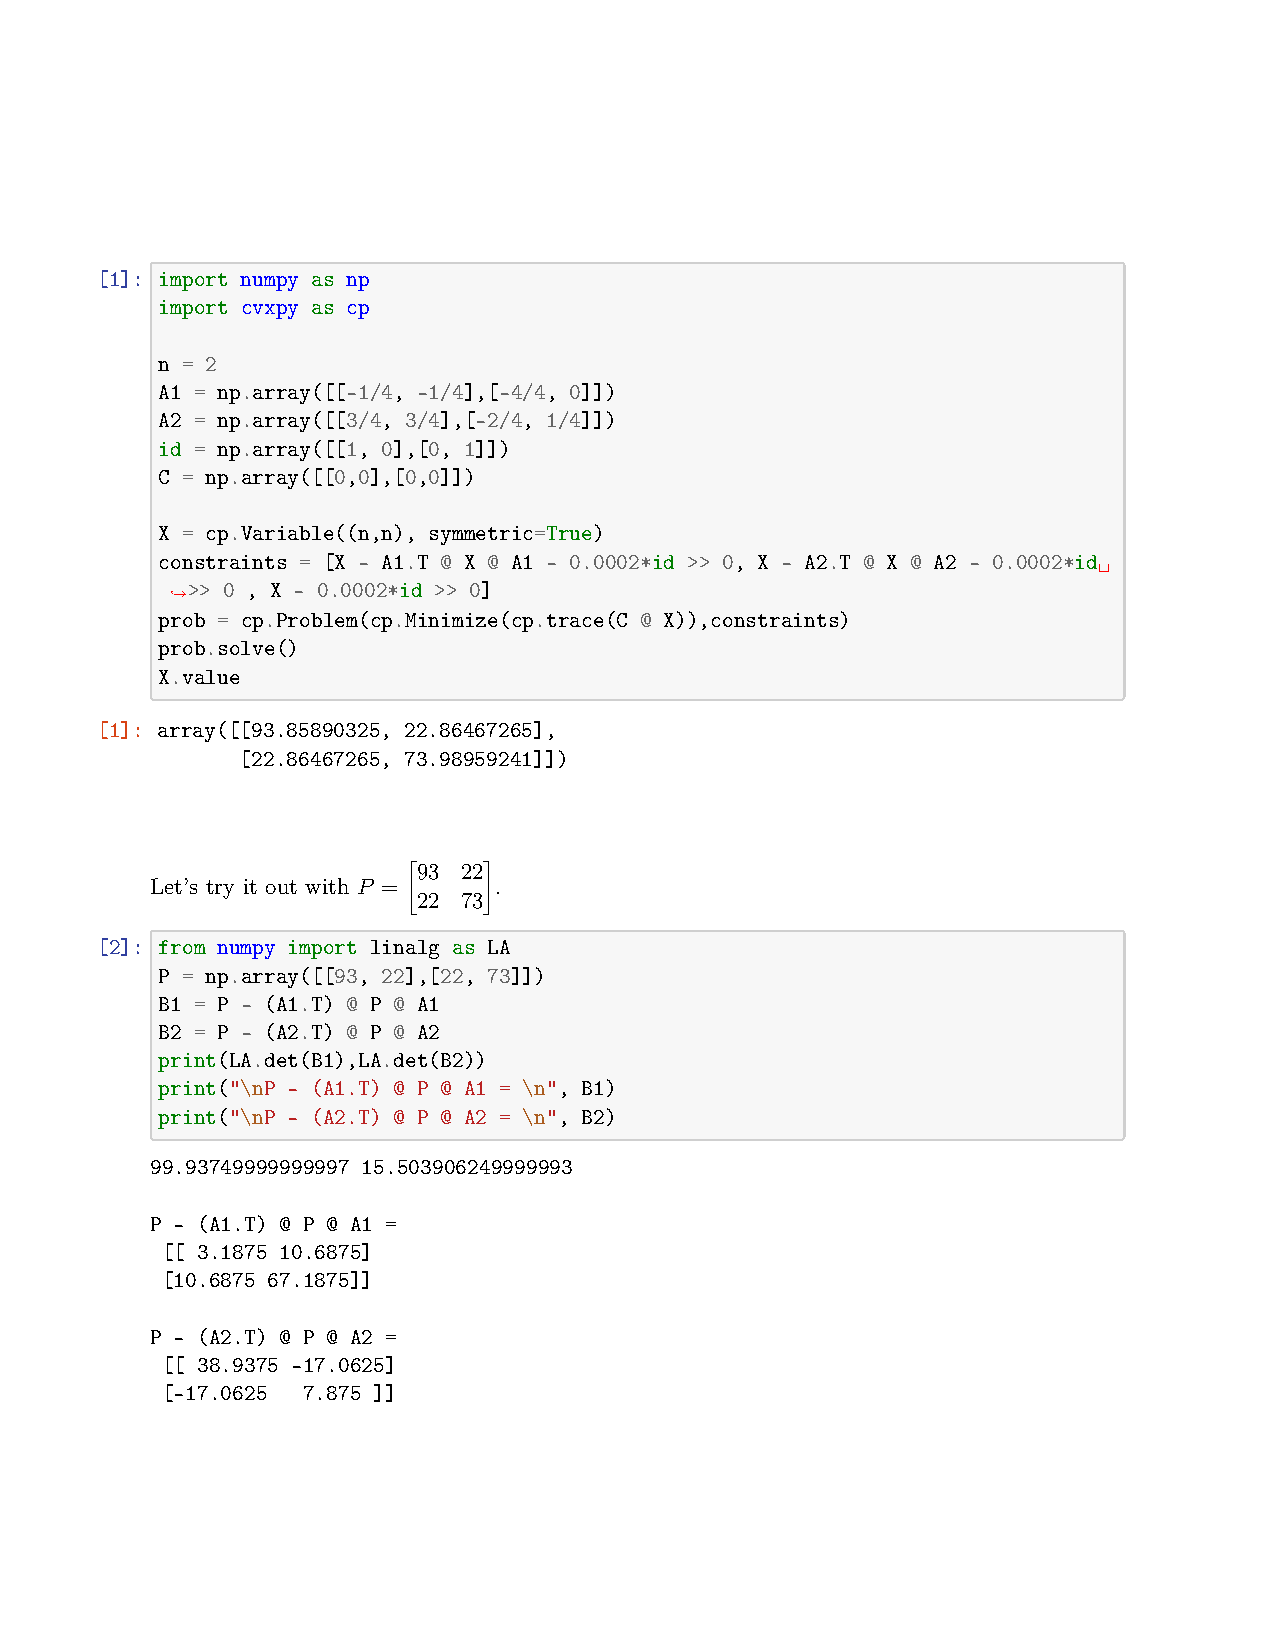
\includepdf[pages=-,pagecommand={\label{pdf:stab}}]{stability/stab.pdf}}

\end{enumerate}


\newpage
\pb
Give an example of symmetric $n \times n$ matrices $A_{1}, \cdots , A_{m}$ with rational entries and rational numbers $b_{1},\cdots,b_{m}$ such that the set 
$$S = \set{X\in S^{n\times n}\st\Tr(A_{i}X) = b_{i}~\forall 1\le i\le m, X\succeq 0}$$ is non-empty, but only contains matrices that have at least one irrational entry. Here, $S^{n\times n}$ denotes the set of symmetric $n \times n$ matrices with real entries and $\Tr$ stands for the trace operation.

\soln

Recall that if $A,B$ are square matrices then $\begin{bmatrix}A&\pmb 0\\\pmb 0&B\end{bmatrix}\succeq 0$ iff $A\succeq 0$ and $B\succeq 0$. This is because the eigenvalues of this block matrix is the union of the set of eigenvalues of $A$ and those of $B$.

Note the following:
\begin{itemize}
\item $\begin{bmatrix}2x&2\\2&x\end{bmatrix}\succeq 0\iff (x\ge 0\text{ and } 2x^{2}\ge 4) \iff (x\ge 0 \text{ and } x^{2}\ge 2) \iff x\ge \sqrt 2$.
\item $\begin{bmatrix}1&x\\x&2\end{bmatrix}\succeq 0\iff 2-x^{2}\ge 0 \iff -\sqrt 2\le x\le \sqrt 2$.
\end{itemize}

Thus we have the following set if equivalent statements for the matrix $A\sett 
\begin{bmatrix}2x&2 &0 &0\\
2&x&0 &0\\
0&0&1&x\\
0&0&x&2
\end{bmatrix}\in S^{4\times 4}$:
\begin{align*}
&A\succeq 0\\
\iff& \begin{bmatrix}2x&2\\2&x\end{bmatrix}\succeq 0 \text{ and } \begin{bmatrix}1&x\\x&2\end{bmatrix}\succeq 0\\
\iff& x\ge \sqrt 2 \text{ and } -\sqrt 2\le x\le \sqrt 2\\
\iff& x=\sqrt2.
\end{align*}
Now it remains to put linear constraints on $X\in S^{4\times 4}$ so that it takes the form of $A$ with $x$ variable. This is obtained as follows (we denote $\Tr(CX) = C*X$):
\begin{multicols}{3}\begin{enumerate}
\item $\begin{bmatrix}
0&0 &1 &0\\
0&0&0 &0\\
1&0&0&0\\
0&0&0&0
\end{bmatrix} \ast X = 0$.
\item $\begin{bmatrix}0&0 &0 &1\\
0&0&0 &0\\
0&0&0&0\\
1&0&0&0
\end{bmatrix} \ast X = 0$.
\item $\begin{bmatrix}
0&0 &0 &0\\
0&0&1 &0\\
0&1&0&0\\
0&0&0&0
\end{bmatrix} \ast X = 0$.
\item $\begin{bmatrix}0&0 &0 &0\\
0&0&0 &1\\
0&0&0&0\\
0&1&0&0
\end{bmatrix}\ast X = 0$.
\item $\begin{bmatrix}
0&1 &0 &0\\
1&0&0 &0\\
0&0&0&0\\
0&0&0&0
\end{bmatrix}\ast X = 4$. 
\item $\begin{bmatrix}
0&0 &0 &0\\
0&0&0 &0\\
0&0&1&0\\
0&0&0&0
\end{bmatrix}\ast X = 1$.
\item $\begin{bmatrix}
0&0 &0 &0\\
0&0&0 &0\\
0&0&0&0\\
0&0&0&1
\end{bmatrix}\ast X = 2$.
\item $\begin{bmatrix}
-1&0 &0 &0\\
0&0&0 &0\\
0&0&0&1\\
0&0&1&0
\end{bmatrix}\ast X = 0$.
\item $\begin{bmatrix}
-1&0 &0 &0\\
0&2&0 &0\\
0&0&0&0\\
0&0&0&0
\end{bmatrix}\ast X = 0$.
\end{enumerate}\end{multicols}

We make a table to show what $X$ looks like, after the above linear constraints are taken into account.

% Please add the following required packages to your document preamble:
% \usepackage[table,xcdraw]{xcolor}
% Beamer presentation requires \usepackage{colortbl} instead of \usepackage[table,xcdraw]{xcolor}
\begin{table}[]
\begin{tabular}{|l|p{0.6\textwidth}|l|}
\hline
\rowcolor[HTML]{EFEFEF} 
\multicolumn{1}{|c|}{\cellcolor[HTML]{EFEFEF}\textbf{Step $\#$}} & \multicolumn{1}{c|}{\cellcolor[HTML]{EFEFEF}\textbf{What it does}}                                                              & \multicolumn{1}{c|}{\cellcolor[HTML]{EFEFEF}\textbf{$X$ after this step}} \\ \hline
$1-4$                                                            & Sets the top right $4\times 4$, and hence bottom left, portion to $0$                                                          & $\begin{bmatrix}a&b &0 &0\\b&c&0 &0\\0&0&d&x\\0&0&x&e\end{bmatrix}$       \\ \hline
$5$                                                              & Takes the off-diagonals in the top left $4\times 4$ corner (that is, $b$) and sets their sum to $4$. So $b+b=4\implies b=2$. & $\begin{bmatrix}a&2 &0 &0\\2&c&0 &0\\0&0&d&x\\0&0&x&e\end{bmatrix}$       \\ \hline
$6$                                                              & Sets the top-left entry of the bottom-right $4\times 4$ submatrix to $1$.                                                       & $\begin{bmatrix}a&2 &0 &0\\2&c&0 &0\\0&0&1&x\\0&0&x&e\end{bmatrix}$       \\ \hline
$7$                                                              & Sets the bottom-right entry to $2$.                                                                                             & $\begin{bmatrix}a&2 &0 &0\\2&c&0 &0\\0&0&1&x\\0&0&x&2\end{bmatrix}$       \\ \hline
$8$                                                              & Equates $X_{11} = X_{34}+X_{43} = 2x$.                                                                                          & $\begin{bmatrix}2x&2 &0 &0\\2&c&0 &0\\0&0&1&x\\0&0&x&2\end{bmatrix}$      \\ \hline
$9$                                                              & Equates $X_{22} = \frac{1}{2}X_{11}$.                                                                                           & $\begin{bmatrix}2x&2 &0 &0\\2&x&0 &0\\0&0&1&x\\0&0&x&2\end{bmatrix}$      \\ \hline
\end{tabular}
\end{table}

From the above, it is clear that $n=4, m=9$ and the enumeration gives what the $A_{1},\cdots,A_{m}\in S^{n\times n}$ and $b_{1},\cdots,b_{m}\in \R$ are. There is only one matrix $X\in S^{n\times n}$ which satisfies $A_{i}X=b_{i}~\forall 1\le i\le m$ and $X\succeq0$, namely $\begin{bmatrix}2\sqrt2&2 &0 &0\\2&\sqrt2&0 &0\\0&0&1&\sqrt2\\0&0&\sqrt2&2\end{bmatrix}$.




\end{document}

